desarrollo tecnico
\paragraph{Desarrollo técnico}
El objetivo de este circuito estaba pensado para dar una aplicaci'on a la señal digitalrecibida por el receptor. El circuito consistía en un smith trigger para forzar una señal digital y una máquina de estados cuya salida tenía una aplicación concreta. En este caso, por cada señal recibida, poner en alto una de sus salidas, manteniendo el estado de las anteriores hasta completar el ciclo, donde todas volverían a estado bajo. 
El esquemático del circuito digital de la máquina de estados y el smith trigger se muestran en las figuras REF y REF respectivamente.
Además se añade, en la figura REF, la integración del receptor superheterodino FM anterior, junto al circuito digital.

\begin{figure}[h!]
    \centering
    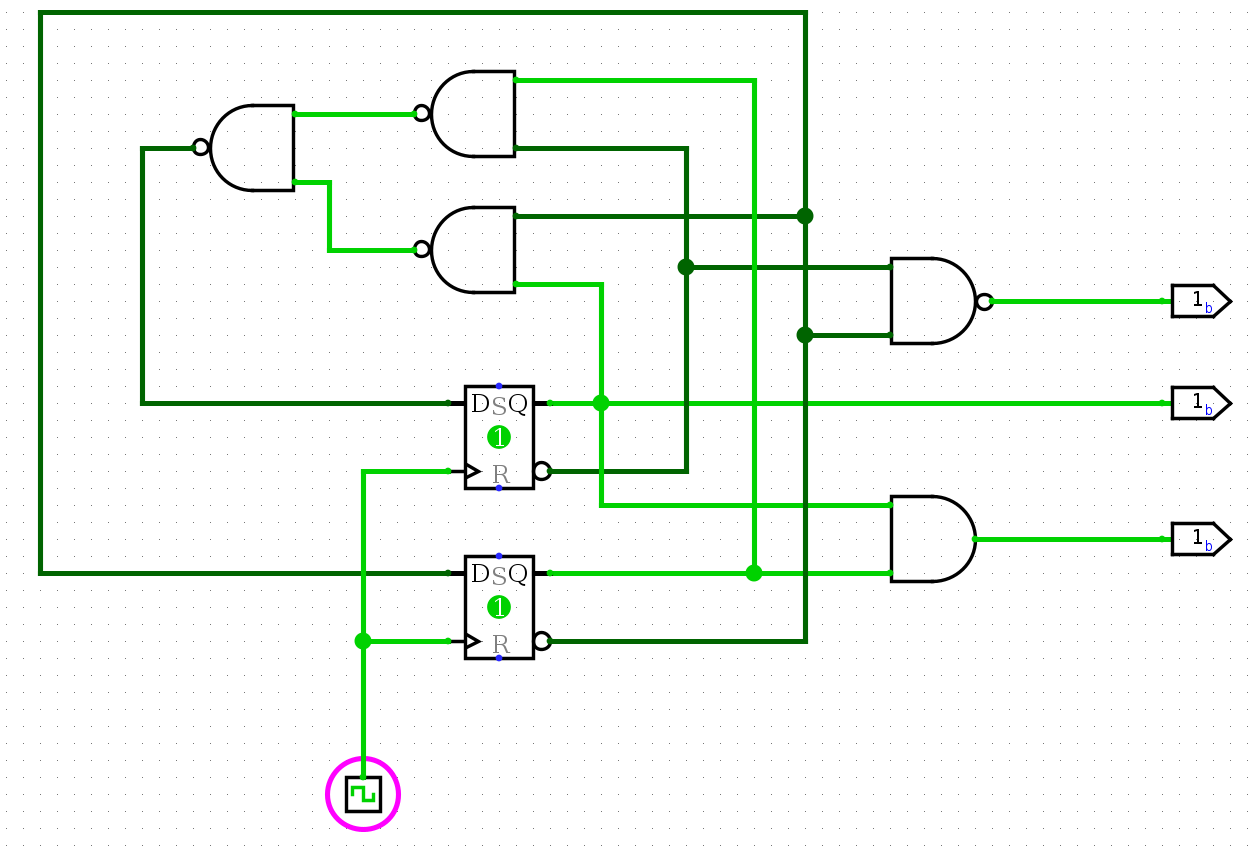
\includegraphics[scale=1, width=.6\textwidth]{crono_logisim}
    \caption{maquina estados esquematico}
    \label{fig:simrx_zoom}
\end{figure}

\begin{figure}[h!]
    \centering
    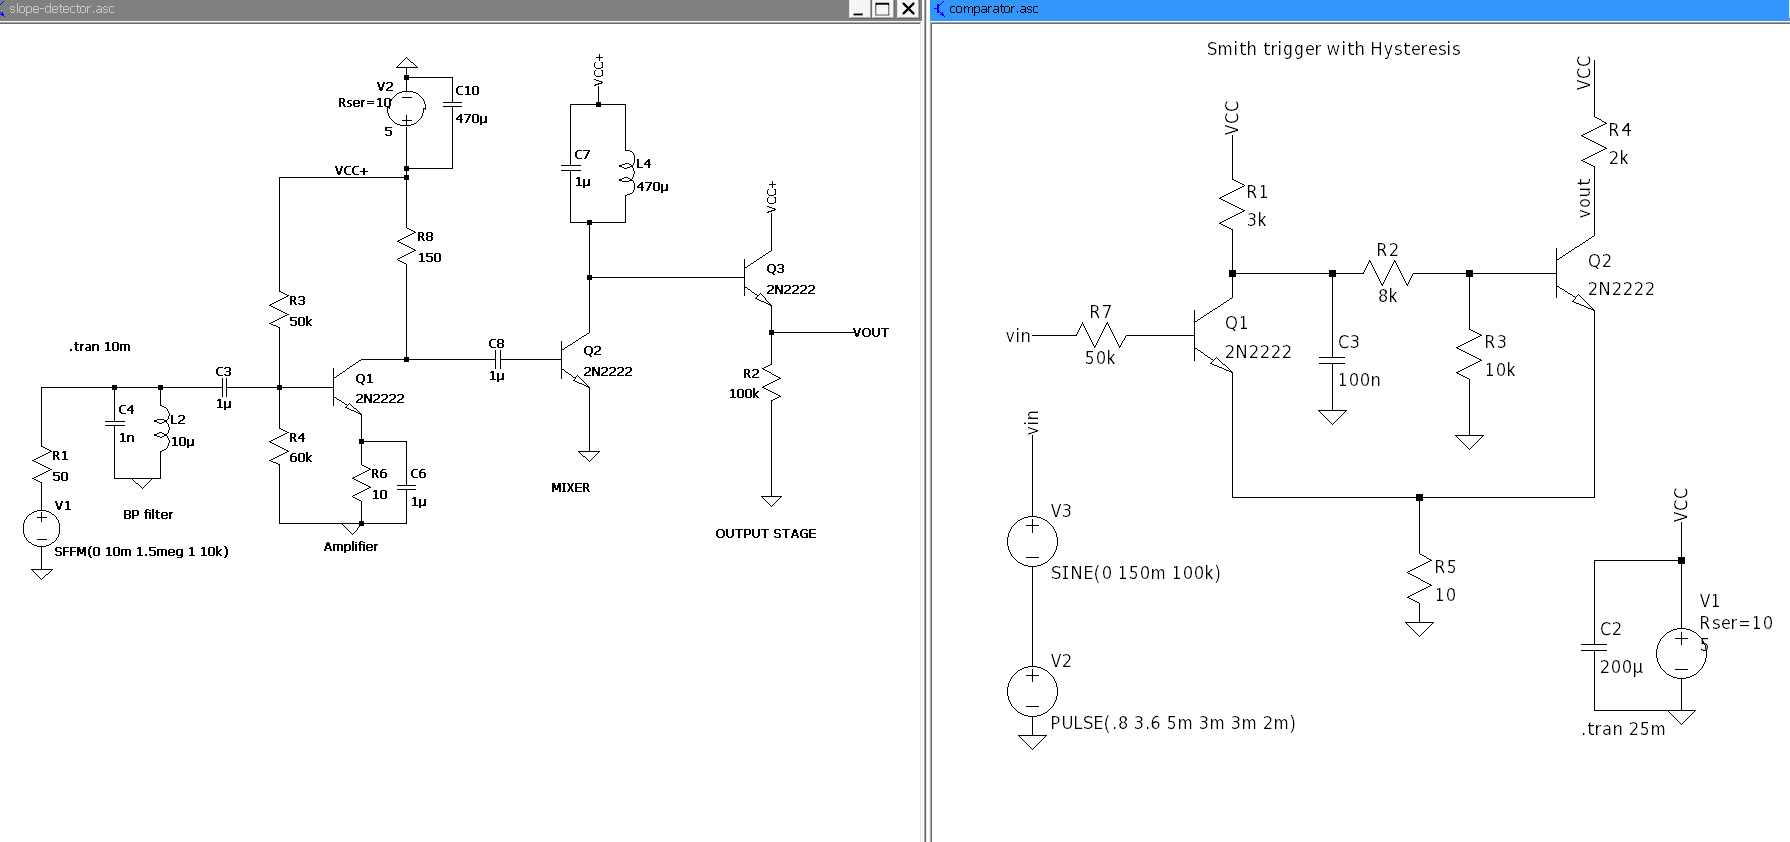
\includegraphics[scale=1, width=1\textwidth]{crono_sch_receiver_varactor}
    \caption{receptor general schematic}
    \label{fig:simrx_zoom}
\end{figure}

\begin{figure}[h!]
    \centering
    \includegraphics[scale=.5, width=.5\textwidth]{crono_general}
    \caption{receptor general real}
    \label{fig:simrx_zoom}
\end{figure}

\paragraph{Motivos de reemplazo}
El diseño del circuito digital era correcto. Sin embargo, al realizar la integración con el receptor daba muchos problemas debido a que la señal de output del receptor no era fiable. Esta señal, al no estar bien filtrada poseía componentes residuales de alta frecuencia que provocaban que el smith trigger metiera señales falsas. esto provocaba un comportamiento no deseado del circuito. 
Para solucionar este hecho, se hizo uso de un microcontrolador. El micro abre una inmensidad de posibilidades como la recepci\'on de múltiples canales, reprogramable en función del uso específico, todo contenido en un menor espacio e incluso con un precio más económico.
